\documentclass[supercite]{Experimental_Report}

\title{~~~~~~数据结构实验~~~~~~}
\author{王李超}
%\coauthor{张三、李四}
\school{计算机科学与技术学院}
\classnum{CS启明2401}
\stunum{U202414887}
%\costunum{U202115631、U202115631}
\instructor{王雄} % 该系列实验报告模板有华科大计院教师陈加忠制作
\date{2025年5月1日}

\usepackage{algorithm, multirow}
\usepackage{algpseudocode}
\usepackage{amsmath}
\usepackage{amsthm}
\usepackage{framed}
\usepackage{mathtools}
\usepackage{fix-cm}
\usepackage{fontspec}
\usepackage{subcaption}
\usepackage{xltxtra} %提供了针对XeTeX的改进并且加入了XeTeX的LOGO, 自动调用xunicode宏包(提供Unicode字符宏)
\usepackage{bm}
\usepackage{tabularx}
\usepackage{ltablex}
\usepackage{tikz}
\usepackage{tikzscale}
\usepackage{pgfplots}
\usepackage{caption}
%\usepackage{enumerate}

\pgfplotsset{compat=1.16}

\newcommand{\cfig}[3]{
  \begin{figure}[htb]
    \centering
    \includegraphics[width=#2\textwidth]{images/#1.tikz}
    \caption{#3}
    \label{fig:#1}
  \end{figure}
}

\newcommand{\sfig}[3]{
  \begin{subfigure}[b]{#2\textwidth}
    \includegraphics[width=\textwidth]{images/#1.tikz}
    \caption{#3}
    \label{fig:#1}
  \end{subfigure}
}

\newcommand{\xfig}[3]{
  \begin{figure}[htb]
    \centering
    #3
    \caption{#2}
    \label{fig:#1}
  \end{figure}
}

\newcommand{\rfig}[1]{\autoref{fig:#1}}
\newcommand{\ralg}[1]{\autoref{alg:#1}}
\newcommand{\rthm}[1]{\autoref{thm:#1}}
\newcommand{\rlem}[1]{\autoref{lem:#1}}
\newcommand{\reqn}[1]{\autoref{eqn:#1}}
\newcommand{\rtbl}[1]{\autoref{tbl:#1}}

\algnewcommand\Null{\textsc{null }}
\algnewcommand\algorithmicinput{\textbf{Input:}}
\algnewcommand\Input{\item[\algorithmicinput]}
\algnewcommand\algorithmicoutput{\textbf{Output:}}
\algnewcommand\Output{\item[\algorithmicoutput]}
\algnewcommand\algorithmicbreak{\textbf{break}}
\algnewcommand\Break{\algorithmicbreak}
\algnewcommand\algorithmiccontinue{\textbf{continue}}
\algnewcommand\Continue{\algorithmiccontinue}
\algnewcommand{\LeftCom}[1]{\State $\triangleright$ #1}

\newtheorem{thm}{定理}[section]
\newtheorem{lem}{引理}[section]

\colorlet{shadecolor}{black!15}

\theoremstyle{definition}
\newtheorem{alg}{算法}[section]

\def\thmautorefname~#1\null{定理~#1~\null}
\def\lemautorefname~#1\null{引理~#1~\null}
\def\algautorefname~#1\null{算法~#1~\null}

\begin{document}

\maketitle

\clearpage

\pagenumbering{Roman}

\tableofcontents[level=2]

\clearpage

\pagenumbering{arabic}

\section{基于顺序存储结构的线性表实现}



\subsection{问题描述}

\subsubsection{实验目的}
通过实验达到:(1)加深对线性表的概念、基本运算的理解;(2)熟练掌握线性表的逻辑结构与物理结构的关系;(3)物理结构采用顺序表,熟练掌握顺序表基本运算的实现。

\subsubsection{具体问题}

在设计线性表时,需要解决以下具体问题:
\begin{itemize}
	\item \textbf{存储结构的选择:} 选择顺序存储结构还是链式存储结构,需权衡存储效率和操作效率。
	\item \textbf{容量的动态扩展:} 当线性表存储空间不足时,如何动态扩展存储容量以容纳更多元素。
	\item \textbf{基本操作的实现:} 包括插入、删除、查找、更新等操作的具体实现及其时间复杂度优化。
	\item \textbf{边界条件处理:} 如何处理空表、满表以及非法操作(如越界访问)等特殊情况。
	\item \textbf{数据类型的通用性:} 设计线性表时,如何支持存储多种数据类型(如整数、浮点数、字符串等)。
	\item \textbf{内存管理:} 如何高效管理内存,避免内存泄漏或冗余分配。
	\item \textbf{算法效率:} 针对不同操作需求,优化算法以提高线性表的整体性能。
\end{itemize}


\subsection{系统设计}

整体系统结构设计方面,本系统采用模块化设计思想,将顺序表的各项操作功能(如初始化、插入、删除、查找、遍历、排序、文件读写等)分别封装为独立的函数,并通过主程序 main01.cpp 提供统一的菜单式交互界面,方便用户进行各类操作。系统支持多顺序表管理,用户可新建、删除、切换和重命名多个顺序表,提升了系统的灵活性和扩展性。各功能模块之间通过头文件(如 def.h、func.h)进行数据类型和函数声明的解耦,便于维护和升级。

数据结构设计方面,核心采用顺序存储结构实现线性表。定义了 SqList 结构体,包含元素指针和当前长度等信息,实现了线性表的基本操作。为支持多顺序表管理,设计了 LISTS 结构体,内部维护一个顺序表数组,每个元素包含一个 SqList 及其名称。元素类型 ElemType 可根据实际需求灵活定义。通过结构体嵌套和指针管理,系统实现了对多个线性表的统一管理和操作,保证了数据的有序性和高效性。整体设计兼顾了功能完整性、易用性和可扩展性。

\subsection{系统实现}

主要说明各个主要函数的实现思想,复杂函数可辅助流程图进行说明,函数和系统实现的源代码放在附录中。

\subsubsection{主要函数实现思想}

\begin{itemize}
    \item \textbf{InitList}:判断线性表是否已存在,若不存在则分配初始空间,初始化长度和容量。
    \item \textbf{DestroyList}:释放线性表空间,并将指针和长度等信息重置,防止内存泄漏。
    \item \textbf{ClearList}:不释放空间,仅将长度归零,实现逻辑清空。
    \item \textbf{ListEmpty}:判断线性表是否存在及是否为空,返回相应状态。
    \item \textbf{ListLength}:返回线性表当前长度,若不存在则返回异常。
    \item \textbf{GetElem}:获取指定位置元素,先判断合法性和存在性。
    \item \textbf{LocateElem}:顺序查找指定元素,返回其逻辑序号,未找到返回0。
    \item \textbf{PriorElem/NextElem}:查找指定元素的前驱或后继,遍历查找并返回相邻元素。
    \item \textbf{ListInsert}:判断插入位置合法性,必要时扩容,移动元素后插入新元素。
    \item \textbf{ListDelete}:判断删除位置合法性,保存被删元素,移动后续元素覆盖。
    \item \textbf{ListTraverse}:顺序输出所有元素,便于调试和展示。
    \item \textbf{MaxSubArray}:实现最大连续子数组和的求解,采用动态规划思想。
    \item \textbf{SubArrayNum}:统计和为指定值的子数组个数,双重循环遍历所有子区间。
    \item \textbf{sortList}:采用冒泡排序对顺序表元素排序。
    \item \textbf{saveListToFile/loadListFromFile}:实现顺序表的文件保存与加载,便于数据持久化。
    \item \textbf{manageMultipleLists}:输出当前所有顺序表及其名称,实现多表管理。
    \item \textbf{AddList/RemoveList/LocateList}:实现多顺序表的添加、删除和查找,支持名称唯一性和内存管理。
\end{itemize}

\subsubsection{部分函数实现方法}

以下选取几个实现较为复杂或具有代表性的函数,简要说明其实现思路,并给出伪代码辅助理解。

\paragraph{1. ListInsert(顺序表插入)}
该函数需判断插入位置是否合法,若空间不足则动态扩容,然后将插入位置及其后的元素依次后移,最后插入新元素。

\begin{shaded*}
\begin{alg}{ListInsert(顺序表插入)}
    \label{alg:ListInsert}
    \begin{algorithmic}
        \Input 顺序表 $L$,插入位置 $i$,元素 $e$
        \Output 插入是否成功
        \If{$L$ 不存在}
            \State \Return INFEASIBLE
        \EndIf
        \State 检查内存分配是否成功
        \For{$j = L.length$ \textbf{downto} $i$}
            \State $L.elem[j] \gets L.elem[j-1]$
        \EndFor
        \State 将元素插入到位置 $i$:$L.elem[i-1] \gets e$
        \State \Return OK
    \end{algorithmic}
\end{alg}
\end{shaded*}

\paragraph{2. ListDelete(顺序表删除)}
首先判断删除位置是否合法,保存被删元素,然后将其后的元素依次前移,最后长度减一。

\begin{shaded*}
\begin{alg}{ListDelete(顺序表删除)}
    \label{alg:ListDelete}
    \begin{algorithmic}
        \Input 顺序表 $L$,删除位置 $i$
        \Output 被删除元素 $e$,删除是否成功
        \If{$L$ 不存在}
            \State \Return INFEASIBLE
        \EndIf
        \State 检查删除位置合法性
        \State $e \gets L.elem[i-1]$
        \For{$j = i$ \textbf{to} $L.length-1$}
            \State $L.elem[j-1] \gets L.elem[j]$
        \EndFor
        \State 顺序表长度减一
        \State \Return OK
    \end{algorithmic}
\end{alg}
\end{shaded*}

\paragraph{3. MaxSubArray(最大连续子数组和)}
采用动态规划思想,遍历数组,记录当前子数组和与最大值。

\begin{shaded*}
\begin{alg}{MaxSubArray(最大连续子数组和)}
    \label{alg:MaxSubArray}
    \begin{algorithmic}
        \Input 顺序表 $L$
        \Output 最大连续子数组和 $maxSum$
        \State $maxSum \gets L.elem[0]$
        \State $currentSum \gets 0$
        \For{$i = 0$ \textbf{to} $L.length-1$}
            \If{$currentSum > 0$}
                \State $currentSum \gets currentSum + L.elem[i]$
            \Else
                \State $currentSum \gets L.elem[i]$
            \EndIf
            \If{$currentSum > maxSum$}
                \State $maxSum \gets currentSum$
            \EndIf
        \EndFor
        \State \Return $maxSum$
    \end{algorithmic}
\end{alg}
\end{shaded*}

\paragraph{4. AddList(多顺序表添加)}
支持批量添加,需判断名称唯一性,动态分配空间,并循环插入元素直到输入0结束。

\begin{shaded*}
\begin{alg}{AddList(多顺序表添加)}
    \label{alg:AddList}
    \begin{algorithmic}
        \Input 多顺序表 $Lists$,新表名称 $ListName$
        \Output 添加是否成功
        \For{每个待添加顺序表}
            \While{名称重复}
                \State 提示重新输入 $ListName$
            \EndWhile
            \If{顺序表数量已达上限}
                \State \Return ERROR
            \EndIf
            \State 分配新表空间,初始化
            \While{输入元素 $e \neq 0$}
                \State 插入 $e$ 到新表
            \EndWhile
            \State 添加成功
        \EndFor
        \State \Return OK
    \end{algorithmic}
\end{alg}
\end{shaded*}

\subsection{系统测试}

\begin{figure}[htb]
	\begin{center}
		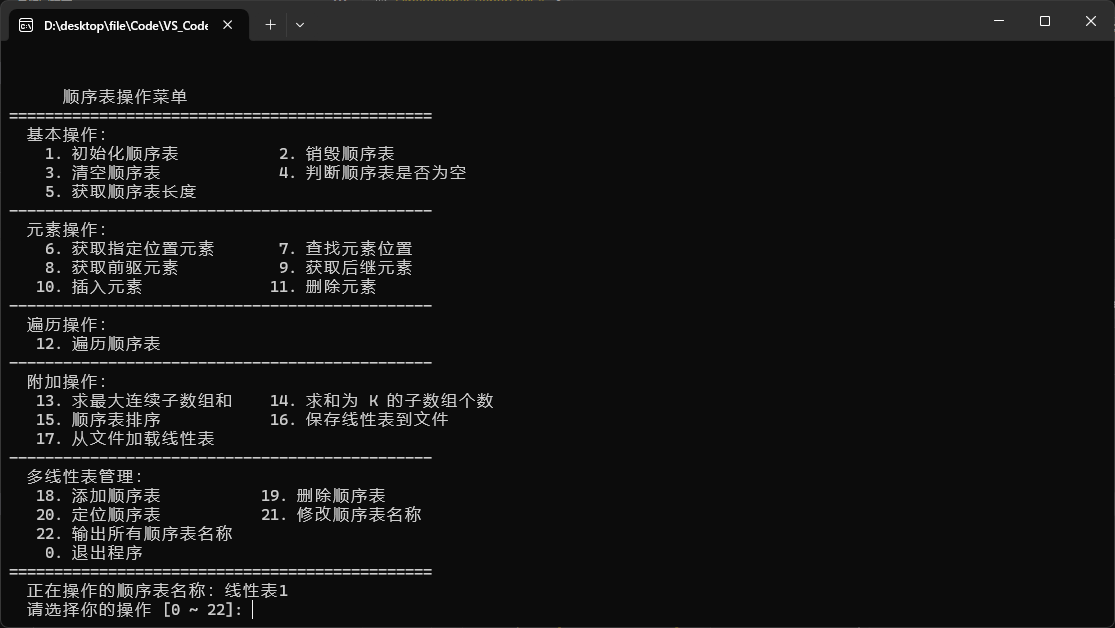
\includegraphics[scale=0.30]{images/1-1.jpg}
		\caption{线性表操作界面}
		\label{fig1-1}
	\end{center}
\end{figure}

主要说明针对各个函数正常和异常的测试用例及测试结果。测试用例设计时,考虑了正常情况、边界条件(如\ref{table:seqlist-test}中多次创建、删除线性表,查询边界处元素)和异常情况等多种场景,确保系统的健壮性和稳定性。以下是部分测试用例及其结果:

\newpage

\subsubsection{基础功能测试}
    \begin{center}
        \setlength{\tabcolsep}{2.0mm}
        \captionof{table}{线性表主要功能测试用例及结果}
        \label{table:seqlist-test}
        \begin{tabularx}{\textwidth}{|X|X|X|}
            \hline
            测试功能及序号 & 输入 & 输出 \\\hline
            1. 构造空线性表 & \textbackslash & 线性表创建成功! \\\hline
            1. 构造空线性表 & \textbackslash & 线性表创建失败! \\\hline
            10. 插入元素(3次) & 4 1;6 2;8 3 & 插入成功!(3次) \\\hline
            4. 判空线性表 & \textbackslash & 线性表不是空表! \\\hline
            5. 求表长 & \textbackslash & 线性表的长度为:3 \\\hline
            6. 获取元素 & 2 & 线性表的第2个元素为:6 \\\hline
            7. 定位元素 & 8 & 线性表中元素8的序号为:3 \\\hline
            8. 获取前驱 & 4 & 线性表中元素4的前驱元素查找失败! \\\hline
            8. 获取前驱 & 6 & 线性表中元素6的前驱元素为:4 \\\hline
            9. 获取后继 & 8 & 线性表中元素8的后继元素查找失败! \\\hline
            9. 获取后继 & 4 & 线性表中元素4的后继元素为:6 \\\hline
            12. 遍历线性表 & \textbackslash & 4 6 8 \\\hline
            16. 文件保存/17. 文件读取 & \textbackslash & 保存成功!/载入成功! \\\hline
            11. 删除元素 & 2 & 线性表中元素6删除成功! \\\hline
            3. 清空线性表 & \textbackslash & 线性表清空成功! \\\hline
            2. 销毁线性表 & \textbackslash & 线性表销毁成功! \\\hline
            2. 销毁线性表 & \textbackslash & 线性表销毁失败! \\\hline
            0. 退出系统 & \textbackslash & 欢迎再次使用本系统! \\\hline
        \end{tabularx}
    \end{center}

\begin{figure}[htb]
	\begin{center}
		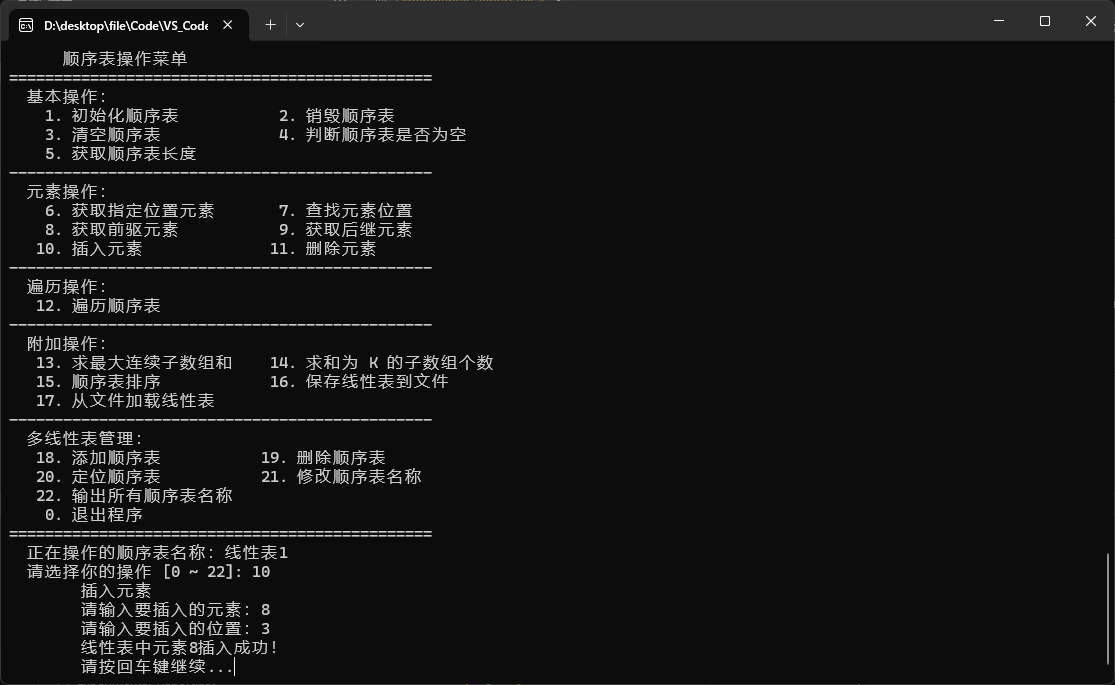
\includegraphics[scale=0.30]{images/1-2.jpg}
		\caption{基础功能测试截图}
		\label{fig1-2}
	\end{center}
\end{figure}

\subsubsection{附加功能测试}

    \begin{center}
        \setlength{\tabcolsep}{2.0mm}
        \captionof{table}{测试时初始状态}
        \label{table:start-status}
        \begin{tabularx}{\textwidth}{|X|X|}
            \hline
            表名称 & 数据 \\\hline
            a & 无  \\\hline
            b & 20 1 2 -4 10 -19 2 2 50  \\\hline
        \end{tabularx}

        \setlength{\tabcolsep}{2.0mm}
        \captionof{table}{线性表附加功能测试用例及结果}
        \label{table:more-seqlist-test}
        \begin{tabularx}{\textwidth}{|X|X|X|}
            \hline
            测试功能及序号 & 输入 & 输出 \\\hline
            13. 最大连续子数组和 & b & 最大连续子数组和为:55 \\\hline
            14. 和为指定值的子数组个数 & 1 2 -3 4 -5 6 7 -8 9 10 & 和为指定值的子数组个数为:0 \\\hline
            15. 顺序表排序 & b & 排序成功! \\\hline
            12. 遍历线性表 & \textbackslash & 20 1 2 -4 10 -19 2 2 50 \\\hline
            16. 文件保存 & \textbackslash & 保存成功! \\\hline
            3. 清空线性表 & \textbackslash & 线性表清空成功! \\\hline
            17. 文件读取 & \textbackslash & 载入成功! \\\hline
            12. 遍历线性表 & \textbackslash & 20 1 2 -4 10 -19 2 2 50 \\\hline
            22. 输出所有顺序表名称 & \textbackslash & 线性表名称:a b \\\hline
        \end{tabularx}
    \end{center}

\begin{figure}[htb]
	\begin{center}
		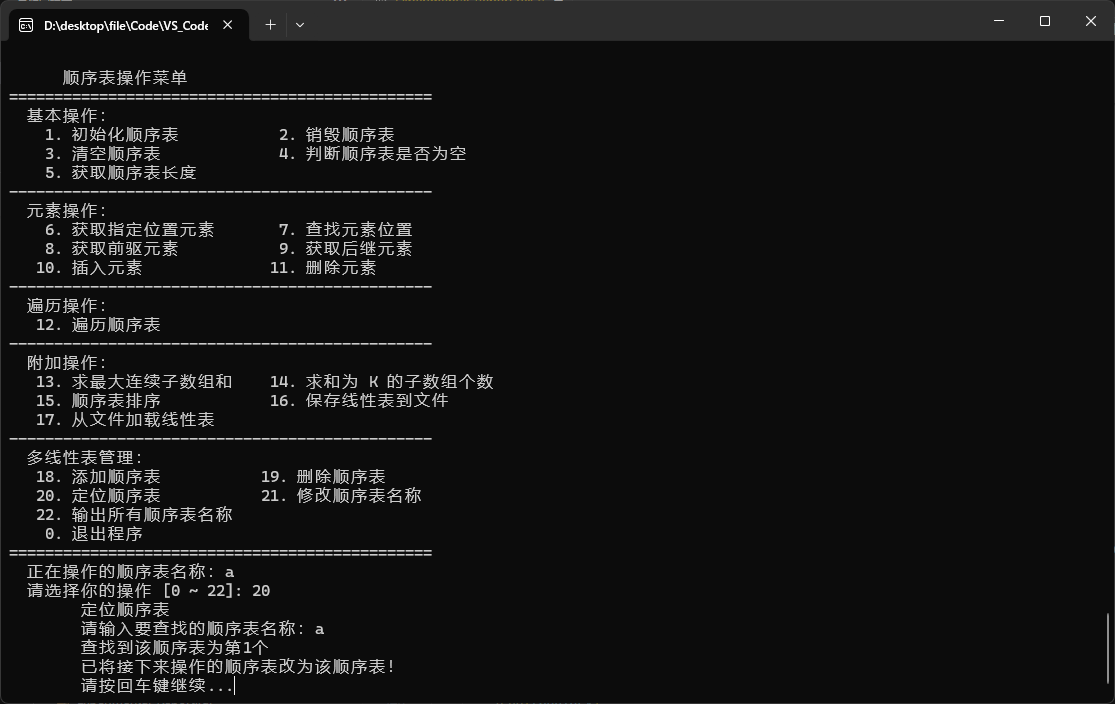
\includegraphics[scale=0.30]{images/1-3.jpg}
		\caption{附加功能测试截图}
		\label{fig1-3}
	\end{center}
\end{figure}

\subsubsection{多线性表管理功能测试}
    \begin{center}
        \setlength{\tabcolsep}{2.0mm}
        \captionof{table}{多线性表管理功能测试用例及结果}
        \label{table:multi-seqlist-test}
        \begin{tabularx}{\textwidth}{|X|X|X|}
            \hline
            测试功能及序号 & 输入 & 输出 \\\hline
            18. 添加线性表 & 2, a, b, 20 1 2 -4 10 -19 2 2 50 0 & 添加成功!(2次) \\\hline
            19. 删除线性表 & 线性表2 & 删除成功! \\\hline
            20. 定位线性表 & 线性表1 & 查找成功! \\\hline
            22. 输出所有顺序表名称 & \textbackslash & a, b \\\hline
            5. 重命名线性表 & a, a1 & 重命名成功! \\\hline
            22. 输出所有顺序表名称 & \textbackslash & a1, b \\\hline
            0. 退出系统 & \textbackslash & 欢迎再次使用本系统! \\\hline
        \end{tabularx}
    \end{center}

\begin{figure}[htb]
	\begin{center}
		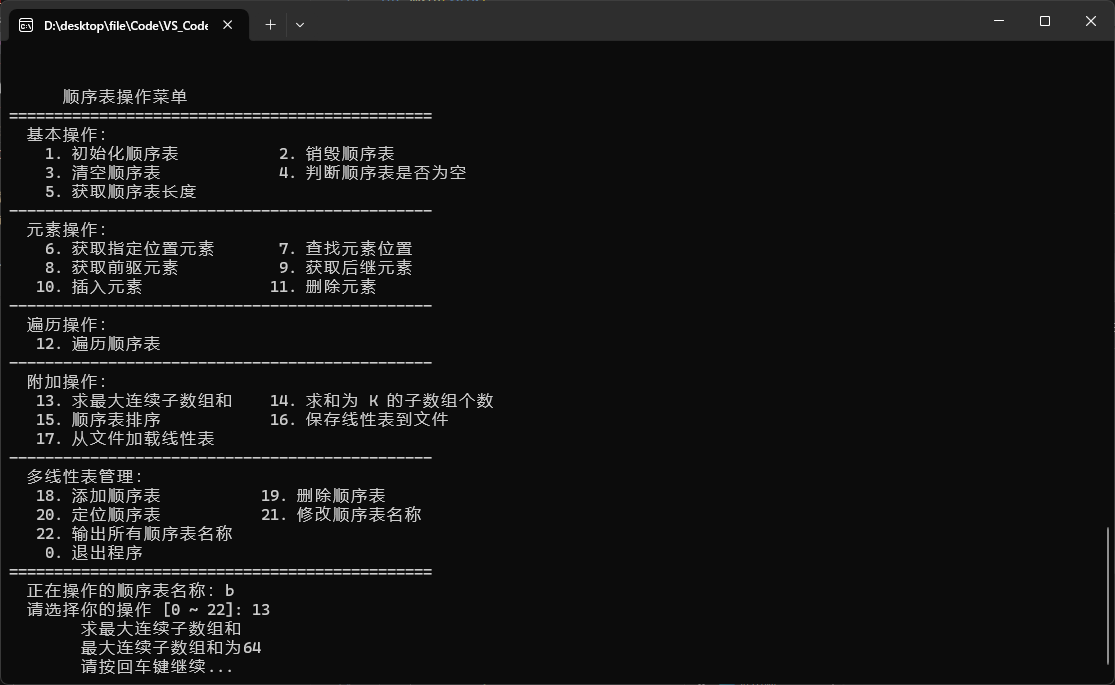
\includegraphics[scale=0.30]{images/1-4.jpg}
		\caption{多线性表管理功能测试截图}
		\label{fig1-4}
	\end{center}
\end{figure}

\subsection{实验小结}

本次实验通过对线性表的实现与操作,深入理解了线性表的基本概念、存储结构及其基本运算。通过对顺序存储结构的实现,掌握了线性表的动态扩展、插入、删除、查找等操作的具体实现方法。同时,通过多顺序表管理功能,提升了系统的灵活性和扩展性。实验中遇到的问题主要集中在内存管理和边界条件处理上,通过不断调试和优化,最终实现了一个功能完整、易用性强的线性表系统。

在设计线性表的过程中,遭遇了一些困难,如如何高效地管理内存、如何处理特殊情况(如空表、满表等)。通过查阅资料和反复测试,逐步解决了这些问题。此外,实验还涉及了文件读写操作的实现,增强了数据的持久化能力。通过对线性表的遍历和排序等操作,提升了系统的实用性和用户体验。整体而言,本次实验不仅加深了对线性表的理解,也提高了编程能力和问题解决能力。

此外,实验还涉及了文件读写操作的实现,增强了数据的持久化能力。通过对线性表的遍历和排序等操作,提升了系统的实用性和用户体验。整体而言,本次实验不仅加深了对线性表的理解,也提高了编程能力和问题解决能力。



\newpage

\section{基于邻接表的图实现}

\subsection{问题描述}

说明此实验要解决的基本问题。大力出奇迹!!!参考文献无法显示怎么办?陈老师正在想办法解决!我是参考文献。我是第二小节\cite{Mehrabian1974An}。我是第二小节\cite{Rezaei2014CVPR}。我是第二小节\cite{Ramnath2008IJCV}。

\subsection{系统设计}

包括整体系统结构设计和数据结构设计等。先在文件夹里的bib文件里添加新的参考文献,给每篇参考文献取一个索引的名字,然后再引用比如\cite{AVS2021Neurocom, Rezaei2014CVPR}。请注意书籍、期刊论文、专利等bib条目的格式是不一样的。画图说明网页的整体框架,进行简要的文字描述等。画图说明网页的整体框架,进行简要的文字描述等。画图说明网页的整体框架,进行简要的文字描述等。画图说明网页的整体框架,进行简要的文字描述等。画图说明网页的整体框架,进行简要的文字描述等。画图说明网页的整体框架,进行简要的文字描述等。画图说明网页的整体框架,进行简要的文字描述等。

\subsection{系统实现}

主要说明各个主要函数的实现思想,复杂函数可辅助流程图进行说明,函数和系统实现的源代码放在附录中。画图说明网页的整体框架,进行简要的文字描述等。画图说明网页的整体框架,进行简要的文字描述等。画图说明网页的整体框架,进行简要的文字描述等。画图说明网页的整体框架,进行简要的文字描述等。画图说明网页的整体框架,进行简要的文字描述等。画图说明网页的整体框架,进行简要的文字描述等。画图说明网页的整体框架,进行简要的文字描述等。

\subsection{系统测试}

主要说明针对各个函数正常和异常的测试用例及测试结果画图说明网页的整体框架,进行简要的文字描述等。画图说明网页的整体框架,进行简要的文字描述等。画图说明网页的整体框架,进行简要的文字描述等。画图说明网页的整体框架,进行简要的文字描述等。画图说明网页的整体框架,进行简要的文字描述等。画图说明网页的整体框架,进行简要的文字描述等。画图说明网页的整体框架,进行简要的文字描述等。

\subsection{实验小结}

\newpage

\section{课程的收获和建议}

描述通过学习该专题,有何收获,有何建议,如某专题可适当减少讲授时间、某专题可适当增加讲授内容和时间等。描述通过学习该专题,有何收获,有何建议,如某专题可适当减少讲授时间、某专题可适当增加讲授内容和时间等。描述通过学习该专题,有何收获,有何建议,如某专题可适当减少讲授时间、某专题可适当增加讲授内容和时间等。描述通过学习该专题,有何收获,有何建议,如某专题可适当减少讲授时间、某专题可适当增加讲授内容和时间等。

\subsection{基于顺序存储结构的线性表实现}

描述通过学习计算机基础知识专题,有何收获,有何建议,如某专题可适当减少讲授时间、某专题可适当增加讲授内容和时间等。描述网页的设计和实现过程中遇到的问题及如何解决。描述网页的设计和实现过程中遇到的问题及如何解决。描述网页的设计和实现过程中遇到的问题及如何解决。描述网页的设计和实现过程中遇到的问题及如何解决。描述网页的设计和实现过程中遇到的问题及如何解决。描述网页的设计和实现过程中遇到的问题及如何解决。描述网页的设计和实现过程中遇到的问题及如何解决。描述网页的设计和实现过程中遇到的问题及如何解决。

\subsection{基于二叉链表的二叉树实现}

描述通过学习计算机基础知识专题,有何收获,有何建议,如某专题可适当减少讲授时间、某专题可适当增加讲授内容和时间等。描述通过学习计算机基础知识专题,有何收获,有何建议,如某专题可适当减少讲授时间、某专题可适当增加讲授内容和时间等。


\nocite{*} %% 作用是不对文献进行引用,但可以生成文献列表

\bibliographystyle{Experimental_Report}
\bibliography{Experimental_Report}
\setcounter{secnumdepth}{0}
\appendix

\section{附录A 基于顺序存储结构线性表实现的源程序}

\noindent
/* Linear Table On Sequence Structure */\\
\#include <stdio.h>\\
\#include <malloc.h>\\
\#include <stdlib.h>\\

\noindent
/*---------page 10 on textbook ---------*/\\
\#define TRUE 1\\
\#define FALSE 0\\
\#define OK 1\\
\#define ERROR 0\\
\#define INFEASTABLE -1\\
\#define OVERFLOW -2\\
\newpage
\section{附录D 基于邻接表图实现的源程序}

\end{document}